\documentclass[tikz]{standalone}

\usepackage{tikz}
\usetikzlibrary{automata}

\begin{document}

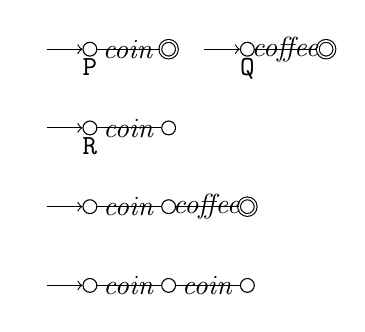
\begin{tikzpicture}
    \tikzstyle{every state}=[
        draw,
        shape=circle,
        inner sep=1pt,
        minimum size=5pt,
        final/.style={double,minimum size=6pt},
        initial text=]
 
    [->,auto,node distance=1.5cm]
    \renewcommand{\a}[1]{\textit{#1}}
    \node[state,initial] (a0) {}; 
    \node[state, final, right of=a0] (a1) {};
    \node[state,initial,right of=a1] (b0) {}; 
    \node[state, final, right of=b0] (b1) {};
    \node[state,initial,below of=a0] (c0) {}; 
    \node[state,        right of=c0] (c1) {};
    \node[state,initial,below of=c0] (n0) {}; 
    \node[state, right of=n0] (n1) {}; 
    \node[state,final,right of=n1] (n2) {};
    \node[state,initial,below of=n0] (m0) {}; 
    \node[state, right of=m0] (m1) {}; 
    \node[state,       right of=m1] (m2) {};
    \path (n0) edge node{\a{coin}} (n1) (n1) edge node{\a{coffee}} (n2)
            (m0) edge node{\a{coin}} (m1) (m1) edge node{\a{coin}} (m2)
            (a0) node[below]{\ttfamily P} (a0) edge node{\a{coin}} (a1)
            (b0) node[below]{\ttfamily Q} (b0) edge node{\a{coffee}} (b1)
            (c0) node[below]{\ttfamily R} (c0) edge node{\a{coin}} (c1);
\end{tikzpicture}
\end{document}